% !TEX encoding = UTF-8 Unicode
\documentclass[a4paper]{article}

\usepackage{color}
\usepackage{url}
\usepackage{amsmath}
\usepackage{csquotes}
\usepackage[T2A]{fontenc} % enable Cyrillic fonts
\usepackage[utf8]{inputenc} % make weird characters work
\usepackage{graphicx}
\usepackage{fullwidth}
\usepackage{float}
\usepackage{caption}
\usepackage{subcaption}
\usepackage[english,serbian]{babel}

\usepackage[unicode]{hyperref}
\hypersetup{colorlinks,citecolor=green,filecolor=green,linkcolor=blue,urlcolor=blue}

\usepackage{listings}
\usepackage{verbatim}
% \usepackage{pseudocode}
\usepackage{algorithm}
\usepackage{algorithmic}
\usepackage{tabularx}
\usepackage{adjustbox}
%\newtheorem{primer}{Пример}[section]
\newtheorem{primer}{Primer}[section]

\definecolor{mygreen}{rgb}{0,0.6,0}
\definecolor{mygray}{rgb}{0.5,0.5,0.5}
\definecolor{mymauve}{rgb}{0.58,0,0.82}



% my commands
\newcommand{\q}[1]{``#1''}  %use this command for quoting
\newcommand{\eng}[1]{(\textit{eng.} #1)}
\floatname{algorithm}{Algoritam}



\lstset{ 
  backgroundcolor=\color{white},   % choose the background color; you must add \usepackage{color} or \usepackage{xcolor}; should come as last argument
  basicstyle=\scriptsize\ttfamily,        % the size of the fonts that are used for the code
  breakatwhitespace=false,         % sets if automatic breaks should only happen at whitespace
  breaklines=true,                 % sets automatic line breaking
  captionpos=b,                    % sets the caption-position to bottom
  commentstyle=\color{mygreen},    % comment style
  deletekeywords={...},            % if you want to delete keywords from the given language
  escapeinside={\%*}{*)},          % if you want to add LaTeX within your code
  extendedchars=true,              % lets you use non-ASCII characters; for 8-bits encodings only, does not work with UTF-8
  firstnumber=1000,                % start line enumeration with line 1000
  frame=single,	                   % adds a frame around the code
  keepspaces=true,                 % keeps spaces in text, useful for keeping indentation of code (possibly needs columns=flexible)
  keywordstyle=\color{blue},       % keyword style
  language=Python,                 % the language of the code
  morekeywords={*,...},            % if you want to add more keywords to the set
  numbers=left,                    % where to put the line-numbers; possible values are (none, left, right)
  numbersep=5pt,                   % how far the line-numbers are from the code
  numberstyle=\tiny\color{mygray}, % the style that is used for the line-numbers
  rulecolor=\color{black},         % if not set, the frame-color may be changed on line-breaks within not-black text (e.g. comments (green here))
  showspaces=false,                % show spaces everywhere adding particular underscores; it overrides 'showstringspaces'
  showstringspaces=false,          % underline spaces within strings only
  showtabs=false,                  % show tabs within strings adding particular underscores
  stepnumber=2,                    % the step between two line-numbers. If it's 1, each line will be numbered
  stringstyle=\color{mymauve},     % string literal style
  tabsize=2,	                   % sets default tabsize to 2 spaces
  title=\lstname                   % show the filename of files included with \lstinputlisting; also try caption instead of title
}

\begin{document}

\title{Pravljenje i optimizacija tima u igri \\
Fantasy Premier League \\ 
\vspace{2mm} \small {Seminarski rad u okviru kursa\\Računarska inteligencija\\ Matematički fakultet}}

\author{Vukašin Radić, Aleksa Voštić\\ vuksain23@gmail.com, akile9v@gmail.com}


%\date{9.~april 2015.}

\maketitle


\abstract{Rešavanje problema pravljenja tima u igri FPL (bench boost varijanta od 15 igrača), korišćenjem i upoređivanjem rezultata različitih algoritama računarske inteligencije.}

\tableofcontents

\newpage


%%%%%%%%%%%%%%%%%%%%%%%%%%%%%%%%%%%%%%%%%%%%%%%%%%%%%%%%%%%%%%%%%%%%%%%%%%%%%%%%%%%%%%%%%%%%%%%%%%%%%%%%%%%%%%%%%
%%%%%%%%%%%%%%%%%%%%%%%%%%%%%%%%%%%%%%%%%%%%%%%%%%%%%%%%%%%%%%%%%%%%%%%%%%%%%%%%%%%%%%%%%%%%%%%%%%%%%%%%%%%%%%%%%
% Pocetak dela (za menjanje pitati autora ovog dela)
% autor: Vukašin Radić
%%%%%%%%%%%%%%%%%%%%%%%%%%%%%%%%%%%%%%%%%%%%%%%%%%%%%%%%%%%%%%%%%%%%%%%%%%%%%%%%%%%%%%%%%%%%%%%%%%%%%%%%%%%%%%%%%
%%%%%%%%%%%%%%%%%%%%%%%%%%%%%%%%%%%%%%%%%%%%%%%%%%%%%%%%%%%%%%%%%%%%%%%%%%%%%%%%%%%%%%%%%%%%%%%%%%%%%%%%%%%%%%%%%


\section{Uvod}
\label{sec:uvod}

Fantasy Premier League je popularna tema istraživanja i analiza iz oblasti optimizacije. Između ostalog, pravljenje i optimizacija tima je jedan od ključnih izazova svakog igrača.

Projekat je realizovan korišćenjem FPL API-a \cite{pythonWrapper} i asyncio module-a \cite{pythonAsyncio}.

\subsection{Pravila Fantasy Premier League igre}
\vspace{3mm}
\label{sec:pravila}
Fantasy Premier League je besplatna online igra u kojoj igrači prave svoj virtuelni tim napravljen od igrača engleske prve lige. Na početku igre, svaki igrač ima na raspolaganju 100.0£ sa kojim mora napraviti virtuelni tim od 15 igrača raznolikih cena. Cilj igre je sakupiti što više bodova tako što igrači predviđaju preformanse svojih virtuelnih igrača u njihovim stvarnim mečevima. Bodovanja se razlikuju od pozicija na kojima su igrači, tako da se za postignute golove, asistencije, sačuvane mreže itd. dobijaju pozitivni poeni, a za promašene penale, autogolove, kartone i primljene golove dobijaju negativni poeni. \\

Pored navedenih ograničenja tima koji ne sme koštati više od 100.0£ (na početku igre) i koji mora brojati 15 virtuelnih igrača, postoje i sledeća:
\begin{enumerate}
  \item Tim ne sme sadržati više od 3 igrača koji igraju u istom klubu
  \item Tim mora sadržati 2 golmana, 5 defanzivaca, 5 veznih igrača i 3 napadača
\end{enumerate} 
\vspace{5mm} %5mm vertical space
Transferi, žetoni, izmene i problem biranja kapitena su deo igre koji ne spada u domen ovog projekta.



\subsection{Cilj projekta}
\vspace{3mm}
Optimizacioni problem kojim se ovaj projekat bavi jeste sastavljanje tima (u skladu sa ograničenjima) tako da se maksimizuje ukupna evaluacija odgovarajućeg tima. Sa obzirom da ne postoji objektivna metrika sa kojom se precizno može oceniti tim, koristili smo se empirijski odabranom kombinacijom parametara i iskustvom vodećih igrača u svetu.  \cite{FPLExpert}. \\

U daljem tekstu su opisana četiri različita pristupa algoritamskom rešavanju zadatog problema, kao i upoređivanje njihovih rezultata i vremena izvršavanja u zavisnosti od veličine ulaznog skupa podataka(igrača).

\vspace{5mm} 


%%%%%%%%%%%%%%%%%%%%%%%%%%%%%%%%%%%%%%%%%%%%%%%%%%%%%%%%%%%%%%%%%%%%%%%%%%%%%%%%%%%%%%%%%%%%%%%%%%%%%%%%%%%%%%%%%
%%%%%%%%%%%%%%%%%%%%%%%%%%%%%%%%%%%%%%%%%%%%%%%%%%%%%%%%%%%%%%%%%%%%%%%%%%%%%%%%%%%%%%%%%%%%%%%%%%%%%%%%%%%%%%%%%
% Kraj dela (za menjanje pitati autora ovog dela)
% autor: Vukašin Radić
%%%%%%%%%%%%%%%%%%%%%%%%%%%%%%%%%%%%%%%%%%%%%%%%%%%%%%%%%%%%%%%%%%%%%%%%%%%%%%%%%%%%%%%%%%%%%%%%%%%%%%%%%%%%%%%%%
%%%%%%%%%%%%%%%%%%%%%%%%%%%%%%%%%%%%%%%%%%%%%%%%%%%%%%%%%%%%%%%%%%%%%%%%%%%%%%%%%%%%%%%%%%%%%%%%%%%%%%%%%%%%%%


%%%%%%%%%%%%%%%%%%%%%%%%%%%%%%%%%%%%%%%%%%%%%%%%%%%%%%%%%%%%%%%%%%%%%%%%%%%%%%%%%%%%%%%%%%%%%%%%%%%%%%%%%%%%%%%%%
%%%%%%%%%%%%%%%%%%%%%%%%%%%%%%%%%%%%%%%%%%%%%%%%%%%%%%%%%%%%%%%%%%%%%%%%%%%%%%%%%%%%%%%%%%%%%%%%%%%%%%%%%%%%%%%%%
% Pocetak dela (za menjanje pitati autora ovog dela)
% autor: Vukašin Radić
%%%%%%%%%%%%%%%%%%%%%%%%%%%%%%%%%%%%%%%%%%%%%%%%%%%%%%%%%%%%%%%%%%%%%%%%%%%%%%%%%%%%%%%%%%%%%%%%%%%%%%%%%%%%%%%%%
%%%%%%%%%%%%%%%%%%%%%%%%%%%%%%%%%%%%%%%%%%%%%%%%%%%%%%%%%%%%%%%%%%%%%%%%%%%%%%%%%%%%%%%%%%%%%%%%%%%%%%%%%%%%%%%%%


\section{Metoda grube sile}

\vspace{3mm} 
Može se primetiti da se problem sastavljanja tima može formulisati kao modifikacija problema ranca (eng. Knapsack problem). Težina predmeta predstavlja cena igrača, dok je cena predmeta dodeljena vrednost igrača. Modifikacija podrazumeva implementiranje ograničenja navedenih u uvodu.

\subsection{Struktura podataka}
\vspace{3mm} 
Svaki čvor u strukturi podataka stablo, sadrži sledeće atribute: \\
\begin{itemize}
	\item \textbf{level} - redni broj nivoa stabla u kom se nalazi čvor
	\item \textbf{weight} - ukupna cena tima
	\item \textbf{value} - ukupna vrednost tima
	\item \textbf{parent} - referenca na roditelja čvora
	\item \textbf{inserted} - indikator da li je igrač ubačen u tim
	\item \textbf{position} - pozicija igrača
	\item \textbf{positionState} - vektor koji predstavlja broj igrača koliko igrača fali na svakoj poziciji ([0,gk,def,mid,att]: [0,2,5,5,3] - tim je prazan, [0,0,0,0,0] - tim je pun)
	\item \textbf{teamsState} -  vektor koji predstavlja broj dostupnih igrača iz svakog kluba, ([0,3...3] - tim je prazan, [0,2,3...1] - uzeti igrači iz klubova čiji je indeks manji od 3) \\
	
	komentar: indeksiranje kreće od 1 radi olakšanog rada sa FPL bibliotekom

\end{itemize}

\subsection{Algoritam}
\vspace{3mm} 

Algoritam funkcioniše po principu pretrage i odsecanje svih svih mogućih kombinacija igrača koji mogu činiti tim. Igrači, sortirani nerastuće po svojim vrednostima, se redom razmatraju da li ispunjavaju uslov za ulazak u tim njihovog čvora roditelja. Binarno stablo pokriva jedine dve mogućnosti, da li je narednog igrača moguće ubaciti u tim ili ne. Nakon pripreme za obe varijante, grananje se izvršava na sledeći način: 

\begin{enumerate}
  \item Ubacivanje tekućeg igrača u tim roditelja ukoliko su ispunjeni uslovi 
  \vspace{1mm}
  \begin{itemize}
	\item Kreiraj novi čvor sa ažuriranim vrednostima nivoa,ukupne cene i vrednosti tima, pozicijom na kojoj igra igrač kao i vrednostima vektora pozicije i klubova.  
	\vspace{1mm}
	\item Ukoliko je pronađena nova maksimalna vrednost tima, ažuriraj je i zapamti čvor kao potencijalno finalan.

	
  \end{itemize}
  \vspace{1mm}
  \item Preskakanje tekućeg igrača 
  \vspace{1mm}
  \begin{itemize}
	\item Kreira se novi čvor sa ažuriranom vrednošću nivoa i precizira da igrač nije odabran, dok se ostale vrednosti preuzimaju od roditelja

	
  \end{itemize}
\end{enumerate} 
\vspace{3mm} 

Po završetku izvršavanja algoritama, pamte se maksimalna vrednost tima kao i poslednji čvor preko čijih se referenci na roditelje rekurzivno dobija odabrani tim.


%%%%%%%%%%%%%%%%%%%%%%%%%%%%%%%%%%%%%%%%%%%%%%%%%%%%%%%%%%%%%%%%%%%%%%%%%%%%%%%%%%%%%%%%%%%%%%%%%%%%%%%%%%%%%%%%%
%%%%%%%%%%%%%%%%%%%%%%%%%%%%%%%%%%%%%%%%%%%%%%%%%%%%%%%%%%%%%%%%%%%%%%%%%%%%%%%%%%%%%%%%%%%%%%%%%%%%%%%%%%%%%%%%%
% Kraj dela (za menjanje pitati autora ovog dela)
% autor: Vukašin Radić
%%%%%%%%%%%%%%%%%%%%%%%%%%%%%%%%%%%%%%%%%%%%%%%%%%%%%%%%%%%%%%%%%%%%%%%%%%%%%%%%%%%%%%%%%%%%%%%%%%%%%%%%%%%%%%%%%
%%%%%%%%%%%%%%%%%%%%%%%%%%%%%%%%%%%%%%%%%%%%%%%%%%%%%%%%%%%%%%%%%%%%%%%%%%%%%%%%%%%%%%%%%%%%%%%%%%%%%%%%%%%%%%



%%%%%%%%%%%%%%%%%%%%%%%%%%%%%%%%%%%%%%%%%%%%%%%%%%%%%%%%%%%%%%%%%%%%%%%%%%%%%%%%%%%%%%%%%%%%%%%%%%%%%%%%%%%%%%%%%
%%%%%%%%%%%%%%%%%%%%%%%%%%%%%%%%%%%%%%%%%%%%%%%%%%%%%%%%%%%%%%%%%%%%%%%%%%%%%%%%%%%%%%%%%%%%%%%%%%%%%%%%%%%%%%%%%
% Pocetak dela (za menjanje pitati autora ovog dela)
% autor: Vukašin Radić
%%%%%%%%%%%%%%%%%%%%%%%%%%%%%%%%%%%%%%%%%%%%%%%%%%%%%%%%%%%%%%%%%%%%%%%%%%%%%%%%%%%%%%%%%%%%%%%%%%%%%%%%%%%%%%%%%
%%%%%%%%%%%%%%%%%%%%%%%%%%%%%%%%%%%%%%%%%%%%%%%%%%%%%%%%%%%%%%%%%%%%%%%%%%%%%%%%%%%%%%%%%%%%%%%%%%%%%%%%%%%%%%%%%


\section{Linearno programiranje}

Pored navedenih metoda, prirodno se nameće i linearno celobrojno programiranje kao jedan od mogućih rešenja zadatog problema. PuLP biblioteka u programskog jeziku Python pruža intuitivan intefejs za formulisanje i rešavanje ove klase problema.

\subsection{Modelovanje problema}

Problem sastavljanja tima se može definisati kao problem maksimizacije zbirne procenjene vrednosti tima. Postupak rešavanja probleme se sastoji iz sledećih koraka:

\begin{enumerate}
  \item \textbf {Definisanje problema} \newline \newline
    Argumenti koje prima konstruktor klase LpProblem kojom modelujemo problem su naziv problema i tip optimizacije   \newline \newline
    \texttt{model = pulp.LpProblem("Team value maximisation", pulp.LpMaximize)}
  \item  \textbf{Uvođenje promenljivih} \newline \newline
  Za svakog igrača iz skupa podataka se pravi zasebna celobrojna promenljiva \textbf{selectedPlayers[i]} koja može uzeti vrednosti 0 ili 1
  \item  \textbf{Funkcija cilja} \newline \newline
  Suma vrednosti odabranih igrača predstavlja vrednost koja se maksimizuje
  \[ \sum_{n=1}^{N}selectedPlayers[i] * players[i].evaluation  \]
  N - veličina skupa \newline
  player.evalation - vrednost tekućeg igrača
  \item  \textbf{Reprezentacija ograničenja} \newline \newline
  Ograničenje budžeta
  \[ \sum_{n=1}^{N}selectedPlayers[i] * \frac{players[i].nowCost}{ 10} \leq 100.0  \] 
  Ograničenje ukupnog broja igrača
  \[ \sum_{n=1}^{N}selectedPlayers = 15  \] \newline
  Ograničenje pozicija: 
  Neka je $k$ oznaka kategorije igrača (koja se čuva u atributu \texttt{elementType} klase \texttt{player}), $I_k$ skup indeksa svih igrača iz kategorije $k$, i $n_k$ traženi broj igrača iz te kategorije.
  Ograničenja pozicija biće oblika:\newline
  \[ (\forall k) \sum_{i \in I_k}selectedPlayers[i] = n_k\]
  Kategorije igrača su sledeće (u zavisnosti od parametra $k$): 1 - golman, 2 - defanzivac, 3 - vezni igrač, 4 - napadač; vrednosti parametra $n_k$ su redom 2, 3, 5, 5, 3.
  \newline
  Ograničenje klubova: Identifikator kluba kome igrač pripada čuva se u polju \texttt{team} klase \texttt{player}. Neka je $C_j$ skup indeksa svih igrača čiji je identifikator kluba jednak $j$. Za svaki klub dodajemo ograničenje oblika:
  \[\sum_{i \in C_j}selectedPlayers[i] \leq 3\]
  \item  \textbf{Rešavanje} \newline \newline
  Pozivanjem metoda \texttt{solve} klase \texttt{LpProblem} biblioteka PuLP pronalazi optimalan rešavač za zadatu formulaciju problema i pokreće ga. Neki od rešavača koje ova biblioteka koristi uključuju CPLEX, GUROBI i COIN\_CMD. Lista dostupnih rešavača dobija se pozivom \texttt{pulp.listSolvers()}.
  \item  \textbf{Tumačenje Rešenja} \newline \newline
  Rešavač će svakoj promenljivoj \texttt{selectedPlayers[i]} dodeliti vrednost 1 ili 0, a finalni tim sastojaće se iz svih promenljivih kojima je dodeljena vrednost 1. Igrači iz finalnog tima se prvo sortiraju po svojoj poziciji, pa se njihova imena i klubovi predstavljaju korisniku zajedno sa njihovom cenom, izraženom u milionima funti. Na kraju se štampaju ukupna cena i vrednost finalnog tima, koji se dobijaju sumiranjem pojedinačnih cena i vrednosti odabranih igrača.
\end{enumerate} 


%%%%%%%%%%%%%%%%%%%%%%%%%%%%%%%%%%%%%%%%%%%%%%%%%%%%%%%%%%%%%%%%%%%%%%%%%%%%%%%%%%%%%%%%%%%%%%%%%%%%%%%%%%%%%%%%%
%%%%%%%%%%%%%%%%%%%%%%%%%%%%%%%%%%%%%%%%%%%%%%%%%%%%%%%%%%%%%%%%%%%%%%%%%%%%%%%%%%%%%%%%%%%%%%%%%%%%%%%%%%%%%%%%%
% Kraj dela (za menjanje pitati autora ovog dela)
% autor: Vukašin Radić
%%%%%%%%%%%%%%%%%%%%%%%%%%%%%%%%%%%%%%%%%%%%%%%%%%%%%%%%%%%%%%%%%%%%%%%%%%%%%%%%%%%%%%%%%%%%%%%%%%%%%%%%%%%%%%%%%
%%%%%%%%%%%%%%%%%%%%%%%%%%%%%%%%%%%%%%%%%%%%%%%%%%%%%%%%%%%%%%%%%%%%%%%%%%%%%%%%%%%%%%%%%%%%%%%%%%%%%%%%%%%%%%


%%%%%%%%%%%%%%%%%%%%%%%%%%%%%%%%%%%%%%%%%%%%%%%%%%%%%%%%%%%%%%%%%%%%%%%%%%%%%%%%%%%%%%%%%%%%%%%%%%%%%%%%%%%%%%%%%
%%%%%%%%%%%%%%%%%%%%%%%%%%%%%%%%%%%%%%%%%%%%%%%%%%%%%%%%%%%%%%%%%%%%%%%%%%%%%%%%%%%%%%%%%%%%%%%%%%%%%%%%%%%%%%%%%
% Pocetak dela (za menjanje pitati autora ovog dela)
% autor: Aleksa Voštić
%%%%%%%%%%%%%%%%%%%%%%%%%%%%%%%%%%%%%%%%%%%%%%%%%%%%%%%%%%%%%%%%%%%%%%%%%%%%%%%%%%%%%%%%%%%%%%%%%%%%%%%%%%%%%%%%%
%%%%%%%%%%%%%%%%%%%%%%%%%%%%%%%%%%%%%%%%%%%%%%%%%%%%%%%%%%%%%%%%%%%%%%%%%%%%%%%%%%%%%%%%%%%%%%%%%%%%%%%%%%%%%%%%%


\section{Genetski Algoritam}
Genetski algoritam je zasnovan na Darvinovoj teoriji evolucije tako da u okviru jedne populacije najčešće opstaju samo najbolje prilagođene jedinke. Nove generacije jedinki se dobijaju ukrštanjem jedinki iz prethodne generacije, uzimajući u obzir da se kod nekih jedinki mogu ponekad dešavati mutacije nad njenim genima. Osnovno očekivanje je da se smenom generacija dobijaju populacije jedinki koje su bolje prilagođene u zadatom okruženju. Svaka jedinka je definisana njenim kôdom koji predstavlja skup njenih gena i na osnovu kojih možemo izračunati pomoću odgovarajuće funkcije prilagođenosti koliko se ta jedinka prilagodila okruženju. Jedinka koja ima najbolju funkciju prilagođenosti možemo smatrati kao najbolji rezultat koji smo dobili primenom genetskog algoritma. Sam algoritam se svodi na nekoliko važnih koraka koji se ponavljaju odgovarajući broj iteracija:
\begin{itemize}
  \item Generisanje početne populacije
  \item Određivanje funkcije prilagođenosti populacije
  \item Sve dok nije ispunjen kriterijum zaustavljanja:
  \begin{itemize}
	\item Izvršiti selekciju jedinki
	\item Ukrstiti izabrane parove jedinki
	\item Potencijalna mutacija izabranih jedinki
	\item Određivanje funkcije prilagođenosti populacije
  \end{itemize}
  \item Ispisivanje najbolje nađenog rešenja.
\end{itemize}

Takođe se može iskoristiti i princip elitizma koji se zasniva na ideji da  se najbolja ili više najboljih jedinki prenesu direktno u narednu generaciju i tako izbegnu slučajevi u kojima najbolja jedinka ne pređe u narednu generaciju ili potomci budu lošiji od roditelja. \cite{genetskiAlgoritamAlicicMatf}. \\


U narednim sekcijama ćemo ukratko opisati na koji način smo svaki od ovih koraka implementirali.

\subsection{Generisanje počene populacije i veličina populacije}
Nakon učitavanja svih fudbalskih igrača koji mogu učestvovati u pravljenju jednog tima, jednu jedinku populacije ćemo definisati kao jedno rešenje koje se sastoji od 15 igrača. Način na koji se vrši izbor igrača koji će činiti jedan tim je totalno proizvoljan, naravno uz poštovanje već navedenih pravila \ref{sec:pravila}. Ovim načinom generisanja početnih jedinki smo hteli da obezbedimo da što više različitih igrača bude izabrano u okviru jedne populacije, jer je broj igrača veliki i na taj način potencijalno obezbedimo raznovrsnije ukrštanje jedinki. Neophodno je i popraviti nekorektnosti kao što su dva ista igrača u okviru jedne iste jedinke, broj igrača na odgovarajućoj poziciji je veći/manji od dozvoljenog i slično.

Veličinu same populacije je jako teško odrediti, jer nam samu jedinku čine diskretni podaci (skup od 15 različitih igrača od oko 600 mogućih), pa je bilo neophodno sprovoditi odgovarajuće testove.\\
Ispostavilo se da za ogromne populacije (>1000), algoritam u većini slučajeva nađe dobro rešenje, što ima i logike: veća veličina populacije daće veću šansu da se prilikom same inicijalizacije u okviru populacije nalazi neko prihvatljivo dobro rešenje, ali to povlači da onda moramo imati i veći broj generacija i samim time algoritam će se duže izvršavati (dok je potencijalno možda već našao dovoljno dobro rešenje). Ovo se isključivo ispostavilo za naš konkretan problem. Nekada je bolje imati veću veličinu populacije nego broj iteracija. \cite{manyGenerations} \\
Za manje vrednosti (<100), algoritam je češće dolazio do lošijih i neprihvatljivijih rešenja. \\
Balans smo našli negde između. Za ne toliko puno vremena i za dovoljno veliku populaciju (oko 500), algoritam daje skroz dobra i prihvaljiva rešenja, a dosta često budu čak i optimalna. \cite{optimalPopulationSize}

\subsection{Određivanje funkcije prilagođenosti populacije}
\label{sec:playerEvaluacija}
Svakoj jedinki računamo prilagođenost na osnovu sledeće formule: 
	\begin{gather*}
		 fitness = \sum_{n=1}^{15 \footnotemark } player.evaluation \\
	\end{gather*}
\footnotetext{Jedna jedinka se sastoji od 15 igrača}
	\begin{gather*}
		\begin{aligned}
		player.evaluation = x*player.total\_points \\ + y*player.form \\ + z*player.selected\_by\_percent \footnotemark \\
		\end{aligned}
	\end{gather*}
\footnotetext{Parametri x,y,z su prilagodljivi i potencijalno će se menjati u zavisnosti od toga čemu želimo da damo više značaja. Važno je da njihov zbir bude jedank 1.0}

Kao što možemo primetiti, na vrlo prost način određujemo prilagođenost jedne jedinke tako što odredimo zbir vrednosti igračevih parametara evaluacije. U ovom slučaju, što je veću vrednost vratila funkcija prilagođenosti jedinke, to nam je rešenje prihvatljivije i bolje. Parametri \textit{total\_points, player.form, player.selected\_by\_percent} su se pokazali kao najbolji za ocenjivanje pojedinačnih igrača koji će činiti jednu jedinku.

\subsection{Kriterijum zaustavljanja}
Algoritam se zaustavlja tek nakon što prođe kroz svaku iteraciju, odnosno dok ne formira i poslednju moguću generaciju. Postavlja se pitanje koji je to optimalan broj generacija koje trebamo proizvesti da bismo došli do optimalnog rešenja? \\ 
Veliki broj iteracija može nam se na prvi pogled činiti kao dobra ideja jer na taj način omogućavamo algoritmu da što više i duže pretražuje oblast pretrage i na taj način pronađe optimalno rešenje, međutim u našem slučaju se to nije ispostavilo kao i najbolja ideja. Veliki broj iteracija (>2000) je definitivno dovodio do boljih i prihvatljivijih rešenja ali ne toliko često i do onog najboljeg rešenja, a uz to se podvlačilo i duže vreme izvršavanja algoritma. \\
Za mali broj iteracija (<300) algoritam je dosta češće nalazio optimalno rešenje za razliku od velikog broja iteracija i to u kratkom vremenskom roku, međutim dosta često je nalazio i lošija rešenja koja možda i nisu toliko prihvatljiva. \\
Zaključili smo da je bolje da imamo dobra i prihvatljivija rešenja, ali i da obezbedimo da imamo šansu da nađemo optimalna rešenja, dok ona lošija na neki način što više zaobiđemo. Zbog toga nismo hteli da uzmemo mali broj iteracija, jer su se češće javljala ne toliko dobra rešenja, od onih koja su prihvatljivija za razliku od velikog broja iteracija gde su se više pojavljivala dobra rešenja ali ne i najbolja. Kao i u određivanju same veličine populacije, balans je negde između. Algoritam nam se najbolje ponaša za izabrani broj iteracija između 500 i 1000. \cite{numOfGener}

\subsection{Selekcija}
Proces selekcije se svodi da u okviru jedne populacije odaberemo neke 2 jedinke da bi kasnije reprodukovali neke nove dve jedinke. Odlučili smo se za turnirsku selekciju jer nam se čini da najbolje pristaje našem problemu. Ideja se svodi na to da iz skupa populacije odaberemo nekoliko jedinki proizvoljno i uvidimo koja jedinka je najbolja od tih nekoliko odabranih, odnosno koja jedinka ima najbolju funkciju prilagođenosti. Na taj način treba odabrati dve takve jedinke i proslediti ih dalje za reprodukovanje novih jedinki. \\
Veličina turnira je postavljena na vrlo malu vrednost jer je algoritam tako davao najbolje rezultate, iako imamo puno jedinki u populaciji. To može biti zbog toga što ukoliko bismo zadali veći turnir, vrlo brzo bismo došli do već nekih ustaljenih lokalnih najboljih rešenja koja bi se stalno takmičila i stalno pobeđivala, pa na taj način ne bismo dozvoljavali nekim drugim jedinkama koje i nisu toliko trenutno prilagodljive, ali možda imaju potencijal da njihova deca budu dosta bolja čak i od tih lokalnih najboljih jedinki. Ispostavilo se da se algoritam najbolje ponašao za veličinu turnira između 3 i 15. Za velike turnire algoritam je vrlo retko nalazio optimalna rešenja, možda 1 u 100 pokretanja, što je vrlo loše.

\subsection{Ukrštanje}
Nakon što procesom selekcije odredimo koje to dve jedinke treba da reprodukuju decu, neophodno je da ih ukrstimo. Ukrštanje se dešava u 100\% slučajeva, odnosno u svakoj iteraciji. Postupak se svodi da prvo sortiramo hromozome oba roditelja po poziciji igrača, tako da dobijemo nešto nalik fudbalskoj formaciji [\textit{gk, gk, df, df, df, df, df, mf, mf, mf, mf, mf, fw, fw, fw}] a nakon toga odaberemo proizvoljni indeks u odnosu na veličinu jedinke (vrednost između 0 i 14) i praktično na tom mestu "presečemo" oba roditelja. Decu formiramo tako što prvi deo prvog roditelja i drugi deo drugog roditelja spojimo za prvo dete i drugi deo prvog roditelja i prvi deo drugog roditelja spojimo za drugo dete. Naravno ovim načinom formiranja novih jedinki često se mogu dešavati nekorektnosti u novo sastavljenom timu, jer prilikom razmene hromozoma, može se desiti da oba roditelja na istoj poziciji imaju istog igrača, pa samim time, jedinka dete koja je nastala njihovim ukrštanjem ima dva ista igrača (npr. dva Salaha u timu), što nije ispravno. Takve i slične probleme neophodno je korektovati. Zbog toga smo uveli i posebnu funkciju korekcije koja nakon ukrštanja, proveri da li je sve dobro prošlo, a ako nije, dodatno izmeni hromozome da bismo dobili korektne vrednosti.

\subsubsection{Korekcija jedinki}
Pošto je problem koji rešavamo poprilično specifičan i ima dosta ograničenja i pravila koje moramo poštovati, morali smo da napravimo odgovarajuću funkciju koja bi mogla da detektuje nekorektnosti i šta više da ih i ispravlja na odgovarajući način. \\
Ideja se svodi da proverimo tri glavna uslova:
\begin{itemize}
	\item Jedinstveni igrači u timu
	\item Ograničenje po broju igrača iz jednog istog tima
	\item Poštovanje budžeta
\end{itemize}

Ukoliko se dogodi bilo koje prekoračenja, algoritam će pomoću funkcije korekcije to detektovati i probati da ustanovi kojeg to igrača treba izbaciti i zameniti ga sa nekim novim proizvoljnim igračem sa iste te pozicije. Nakon toga je naravno opet neophodno da proverimo spomenute uslove, jer mogu biti opet narušeni ubacivanjem novog igrača.

\subsection{Mutacija}
Ideja koja se krije iza mutacije je da se povremeno mogu dešavati neke promene u okviru jedne jedinke koje će promeniti takvu jedinku na samo jednom hromozomu, za razliku od ukrštanja, i na taj način potencijalno podstaći u pronalasku rešenja. \\
Ukoliko je ispunjen uslov da se dogodi mutacija, odabraće se jedan proizvoljan igrač i zameniti sa nekim drugim proizvoljnim igračem sa te iste pozicije u timu. Takođe kao i kod ukrštanja, pozvaće se funkcija koje će nakon mutacije korektovati nepravilnosti koje mogu uslediti ubacivanjem novog igrača u tim. \\
Za naš problem je ustanovljeno da velika stopa mutacije (>0.1) dovodi do eksremno loših rešenja, odnosno ukoliko se mutacija događa često, to će i narušiti već dobro formirane jedinke potencijalnim izbacivanjem i ubacivanjem nekog proizvoljnog igrača. \\
Međutim i niska stopa mutacije (<0.01) se ispostavila poprilično beskorisnim jer algoritam je nalazio solidna rešenja, iako se mutacija događala retko, ali ne i najbolja, pa verovatno možda nije ni podsticala u nalaženju optimalnog rešenja. \\
Treba naglasiti da je mutacija ipak bila možda i presudni faktor kako bi se algoritam ponašao zadovoljavajuće. Ustanovili smo da je stopa mutacije od 0.09 podigla algoritam na dosta viši nivo. Sa ovakvom stopom, algoritam je praktično uspevao da za bilo koje veličine generacije i populacije nalazi u nekoliko pokušaja pokretanja algoritma optimalna rešenja, što za neke manje ili veće vrednosti mutacije nije bio slučaj.

\subsection{Elitizam}
Prilikom pravljenja nove generacije pospukom ukrštanja ili mutacijom, pa kasnije i korektovanjem jedinki, mogu se dešavati situacije u kojima od roditelja koji su dobro prilagođeni dobijamo decu koja su lošije prilagođena od samih roditelja, pa samim time potencijalno ni nema prostora u evoluciji ka najboljem rešenju. Ovo se u našem slučaju može često događati zbog načina na koji je implementirana funkcija korekcija jedinki, pa se zbog toga javila ideja da možda nekoliko najboljih jedinki iz cele populacije direktno prenesemo u narednu generaciju. Iako nam je veličina populacije velika, ispostavilo se da ne trebamo ni previše najboljih jedinki prenositi u narednu generaciju, već samo nekoliko. Ukoliko sačuvamo 1-3 jedinke, algoritam bi se ponašao najbolje.


%%%%%%%%%%%%%%%%%%%%%%%%%%%%%%%%%%%%%%%%%%%%%%%%%%%%%%%%%%%%%%%%%%%%%%%%%%%%%%%%%%%%%%%%%%%%%%%%%%%%%%%%%%%%%%%%%
%%%%%%%%%%%%%%%%%%%%%%%%%%%%%%%%%%%%%%%%%%%%%%%%%%%%%%%%%%%%%%%%%%%%%%%%%%%%%%%%%%%%%%%%%%%%%%%%%%%%%%%%%%%%%%%%%
% Kraj dela (za menjanje pitati autora ovog dela)
% autor: Aleksa Voštić
%%%%%%%%%%%%%%%%%%%%%%%%%%%%%%%%%%%%%%%%%%%%%%%%%%%%%%%%%%%%%%%%%%%%%%%%%%%%%%%%%%%%%%%%%%%%%%%%%%%%%%%%%%%%%%%%%
%%%%%%%%%%%%%%%%%%%%%%%%%%%%%%%%%%%%%%%%%%%%%%%%%%%%%%%%%%%%%%%%%%%%%%%%%%%%%%%%%%%%%%%%%%%%%%%%%%%%%%%%%%%%%%



%%%%%%%%%%%%%%%%%%%%%%%%%%%%%%%%%%%%%%%%%%%%%%%%%%%%%%%%%%%%%%%%%%%%%%%%%%%%%%%%%%%%%%%%%%%%%%%%%%%%%%%%%%%%%%%%%
%%%%%%%%%%%%%%%%%%%%%%%%%%%%%%%%%%%%%%%%%%%%%%%%%%%%%%%%%%%%%%%%%%%%%%%%%%%%%%%%%%%%%%%%%%%%%%%%%%%%%%%%%%%%%%%%%
% Pocetak dela (za menjanje pitati autora ovog dela)
% autor: Aleksa Voštić
%%%%%%%%%%%%%%%%%%%%%%%%%%%%%%%%%%%%%%%%%%%%%%%%%%%%%%%%%%%%%%%%%%%%%%%%%%%%%%%%%%%%%%%%%%%%%%%%%%%%%%%%%%%%%%%%%
%%%%%%%%%%%%%%%%%%%%%%%%%%%%%%%%%%%%%%%%%%%%%%%%%%%%%%%%%%%%%%%%%%%%%%%%%%%%%%%%%%%%%%%%%%%%%%%%%%%%%%%%%%%%%%%%%


\section{Simulirano kaljenje}
Algoritam simuliranog kaljenja \eng{simulated annealing} je zasnovan na procesu kaljenja čelika, čiji je cilj oplemenjivanje metala tako da on postane čvršći. Postepeno hlađenje metala možemo posmatrati kao postupak postepenog smanjivanja verovatnoće da se loše rešenje problema prihvati (u nadi da izbegnemo lokalne ekstremume), kako se prostor rešenja istražuje što znači da se daljom pretragom dolazi do sve optimalnijih rešenja. \\
Zasniva se na poboljšavanju jednog rešenja tako da se u svakom koraku razmatra rešenje u nekoj njegovoj okolini. Na osnovu zadate funkcije cilja, možemo upoređivati rešenja i tako ažurirati trenutno rešenje na bolje rešenje. Ukoliko vrednost funkcije cilja novog rešenja (iz neke okoline) nije bolja od trenutnog rešenja, na osnovu vrednosti odgovarajuća dva parametra \textit{p} i \textit{q} želimo da damo tom slabijem novom rešenju priliku da pronađe sada u njegovoj okolini bolje rešenje i na taj način se potencijalno možemo osloboditi zaglavljivanja u lokalnim ekstremumima. Po potrebi možemo ažurirati i pamtiti vrednost najboljeg dostignutog rešenja. Algoritam se ponavlja sve dok nije ispunjen kriterijum zaustavljanja koji je u najčešćem slučaju maksimalni broj iteracija. \cite{simuliranoKaljenjeAlicicMatf}

\subsection{Generisanje početnog rešenja}
Ustaljeni postpupak generisanja početnog rešenja se svodi na to da pronađemo neko proizvoljno početno rešenje i ispitujemo njegovu okolinu. Zbog specifičnosti našeg problema, ovaj način generisanja se ispostavio poprilično neefikasnim i zbog toga smo morali da primenimo nešto pametniji pristup. \\
Ideja se svodi da početno rešenje generišemo backtracking pristupom \cite{backtrackingMatfMaric}, odnosno napravimo dovoljno kompetativan tim (gledajući njegovu funkciju cilja) i na osnovu njega započnemo dalju pretragu. \\
Postupak se svodi da podelimo sve igrače u 4 liste po pozicijama i svaku listu \textbf{sortiramo} u opadajućem poretku na osnovu parametara evaluacije igrača \ref{sec:playerEvaluacija}. Nakon toga primenom backtracking algoritma počevši od pozicije napadača započnemo formiranje tima tako da uzimamo po jednog igrača, proverimo da li možemo da sastavimo tim sa ovim izabranim igračem tako što mu pridružimo najgore ocenjene igrače na ostalim nepopunjenim pozicijama. Ukoliko je to izvodljivo, nastavljamo dalje dodavanje igrača, ali sa neke druge pozicije iz onih sortiranih lista tako da uzimamo uvek sledećeg najboljeg. Ukoliko nije moguće sastaviti tim od pridodatog igrača i najlošijih igrača, onda tog dodatog igrača ne možemo uzeti u formiranje tima i gledamo ka sledećem igraču u listi nakon njega.

\subsection{Algoritam}
Nakon generisanja početnog rešenja, takvo rešenje ćemo na početku smatrati najboljim i od njega ćemo započeti dalju pretragu. \\
Algoritam se ponavlja n iteracija, mi smo odabrali vrednost oko 100000 jer nema potrebe usporavati algoritam velikim brojem iteracija. Sam problem koji rešava je poprilično težak za algoritam ovakvih sposobnosti zbog raznovrsnosti igrača koji mogu ući u sastavljanje tima. \\
U svakoj iteraciji pokušavamo da nađemo neko susedno rešenje tako što izbacimo nekog proizvoljnog igrača i zamenimo ga sa novim prozivoljnim igračem sa iste pozicije. Ukoliko je funkcija cilja novog rešenja bolja od trenutnog, trenutno rešenje postavljamo na to novo nađeno, a ukoliko nije bolja, onda sa odgovarajućom verovatnoćom mu možemo dati šansu da ipak to lošije rešenje postane trenutno rešenje od kojeg će se odvijati dalja pretraga u narednim iteracijama. Takođe ono što radimo u svakoj iteraciji jeste da pamtimo do sada nađeno najbolje rešenje, zbog toga što algoritam može ponekad da odluta ukoliko damo šansu nekom slabijem rešenju i ne uspe da se vrati ili pronađe neka bolja rešenja kasnije. \\
Nakon završetka i poslednje iteracije, krajnje rešenje je ono rešenje koje se nalazi zapamćeno u najboljem rešenju.


%%%%%%%%%%%%%%%%%%%%%%%%%%%%%%%%%%%%%%%%%%%%%%%%%%%%%%%%%%%%%%%%%%%%%%%%%%%%%%%%%%%%%%%%%%%%%%%%%%%%%%%%%%%%%%%%%
%%%%%%%%%%%%%%%%%%%%%%%%%%%%%%%%%%%%%%%%%%%%%%%%%%%%%%%%%%%%%%%%%%%%%%%%%%%%%%%%%%%%%%%%%%%%%%%%%%%%%%%%%%%%%%%%%
% Kraj dela (za menjanje pitati autora ovog dela)
% autor: Aleksa Voštić
%%%%%%%%%%%%%%%%%%%%%%%%%%%%%%%%%%%%%%%%%%%%%%%%%%%%%%%%%%%%%%%%%%%%%%%%%%%%%%%%%%%%%%%%%%%%%%%%%%%%%%%%%%%%%%%%%
%%%%%%%%%%%%%%%%%%%%%%%%%%%%%%%%%%%%%%%%%%%%%%%%%%%%%%%%%%%%%%%%%%%%%%%%%%%%%%%%%%%%%%%%%%%%%%%%%%%%%%%%%%%%%%




%%%%%%%%%%%%%%%%%%%%%%%%%%%%%%%%%%%%%%%%%%%%%%%%%%%%%%%%%%%%%%%%%%%%%%%%%%%%%%%%%%%%%%%%%%%%%%%%%%%%%%%%%%%%%%%%%
%%%%%%%%%%%%%%%%%%%%%%%%%%%%%%%%%%%%%%%%%%%%%%%%%%%%%%%%%%%%%%%%%%%%%%%%%%%%%%%%%%%%%%%%%%%%%%%%%%%%%%%%%%%%%%%%%
% Pocetak dela (za menjanje pitati autora ovog dela)
% autor: Vukašin Radić, Aleksa Voštić
%%%%%%%%%%%%%%%%%%%%%%%%%%%%%%%%%%%%%%%%%%%%%%%%%%%%%%%%%%%%%%%%%%%%%%%%%%%%%%%%%%%%%%%%%%%%%%%%%%%%%%%%%%%%%%%%%
%%%%%%%%%%%%%%%%%%%%%%%%%%%%%%%%%%%%%%%%%%%%%%%%%%%%%%%%%%%%%%%%%%%%%%%%%%%%%%%%%%%%%%%%%%%%%%%%%%%%%%%%%%%%%%%%%

\section{Analiza rezultata}

Testiranje se obavilo na konfiguraciji:
\vspace{3mm} 
\begin{itemize}
	\item AMD Ryzen 5 3550H with Radeon Vega Mobile Gfx, 2100 Mhz, 4 Core(s), 8 Logical Processor(s)
	\item 12.0GB RAM @933MHz
	\item 476GB SSD Hitachi hfm512gdhtng-8310a 
	\item Windows 10 Enterprise 64-bit

\end{itemize}



\subsection{Metoda grube sile i Linearno programiranje}

Za ekvivalentne skupove ulaznih podataka očekivano se dobijaju isti rezultati pri izvršavanju oba algoritma (Slika 1). Značajno se razlikuje vreme izvršavanje izraženo u sekundama. (Slika 2). 


\begin{figure}[H]
    \centering
    \begin{subfigure}{0.6\textwidth}
    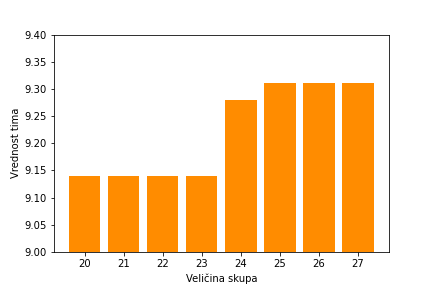
\includegraphics[width = \textwidth]{img/performance_bar.png}
    \end{subfigure}
    \caption{Kvalitet ocene u zavisnosti od veličine skupa}
\end{figure}

\begin{figure}[H]
    \centering
    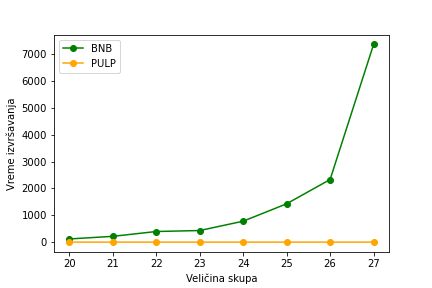
\includegraphics[scale=0.5]{img/exectimes.png}
    \caption{Vreme izvršavanja (sekunde) u zavisnosti od veličine skupa (broj igrača)}
    \label{fig:fig1}
\end{figure}

\subsection{Genetski algoritam i Simulirano kaljenje}

Empirijski odabranim parametrima za Genetski algoritam (veličina populacija: 450 i broj iteracija: 1000 ) i Simulirano kaljenje ( broj iteracija: 100000), dobijeni su sledeći rezultati (Slika 3. i Slika 4.). Može se zaključiti da je Genetski algoritam konzistentnije dobijao veću vrednost (u nekim iteracijama i optimalnu). Simulirano kaljenje se brže izvršavalo ali po ceni lošijih rezultata i ne dostizanja optimimuma.


\begin{figure}[H]
    \centering
    \begin{subfigure}{0.49\textwidth}
    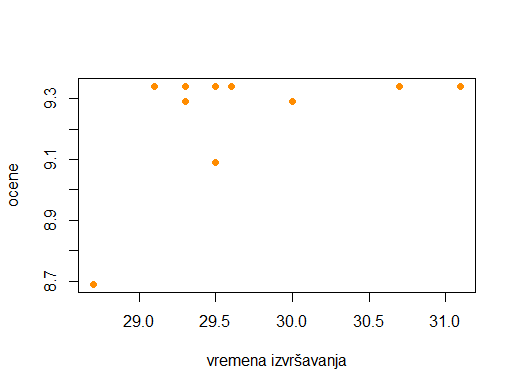
\includegraphics[width = \textwidth]{img/genetski_plot.png}
    \end{subfigure}
    \hfill
    \begin{subfigure}{0.49\textwidth}
    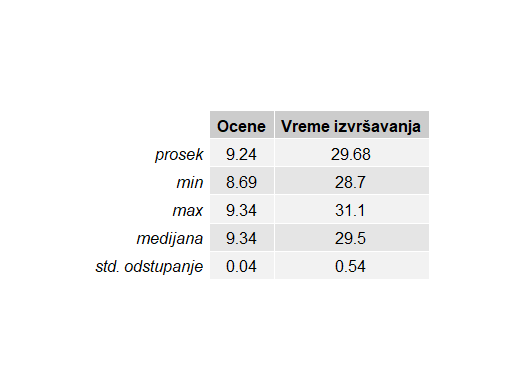
\includegraphics[width = \textwidth]{img/genetski_tabela.png}
    \end{subfigure}
    \caption{Ponašanje genetskog algoritma}
    \label{fig:my_label}
    \centering
    \begin{subfigure}{0.49\textwidth}
    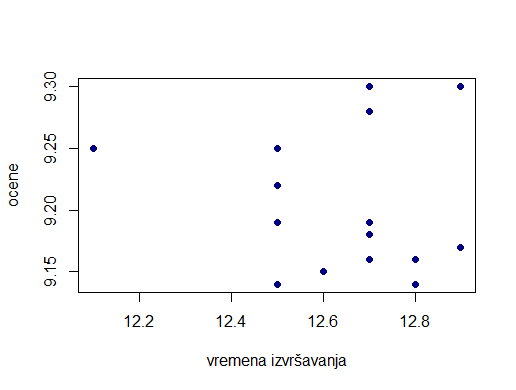
\includegraphics[width = \textwidth]{img/kaljenje_plot.png}
    \end{subfigure}
    \hfill
    \begin{subfigure}{0.49\textwidth}
    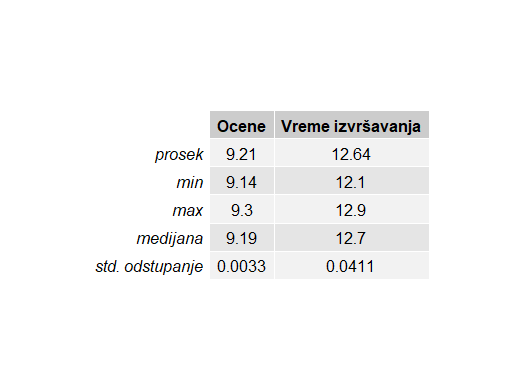
\includegraphics[width = \textwidth]{img/kaljenje_tabela.png}
    \end{subfigure}
    \caption{Ponašanje algoritma simuliranog kaljenja}
    \label{fig:my_label}
\end{figure}

\begin{figure}[H]

\end{figure}



%%%%%%%%%%%%%%%%%%%%%%%%%%%%%%%%%%%%%%%%%%%%%%%%%%%%%%%%%%%%%%%%%%%%%%%%%%%%%%%%%%%%%%%%%%%%%%%%%%%%%%%%%%%%%%%%%
%%%%%%%%%%%%%%%%%%%%%%%%%%%%%%%%%%%%%%%%%%%%%%%%%%%%%%%%%%%%%%%%%%%%%%%%%%%%%%%%%%%%%%%%%%%%%%%%%%%%%%%%%%%%%%%%%
% Kraj dela (za menjanje pitati autora ovog dela)
% autor: Vukašin Radić, Aleksa Voštić
%%%%%%%%%%%%%%%%%%%%%%%%%%%%%%%%%%%%%%%%%%%%%%%%%%%%%%%%%%%%%%%%%%%%%%%%%%%%%%%%%%%%%%%%%%%%%%%%%%%%%%%%%%%%%%%%%
%%%%%%%%%%%%%%%%%%%%%%%%%%%%%%%%%%%%%%%%%%%%%%%%%%%%%%%%%%%%%%%%%%%%%%%%%%%%%%%%%%%%%%%%%%%%%%%%%%%%%%%%%%%%%%

\addcontentsline{toc}{section}{Literatura}
\appendix
\bibliography{seminarski} 
\bibliographystyle{plain}

%\appendix


\end{document}
